\documentclass[crop,tikz]{standalone}
\usepackage{scalerel}

\begin{document}
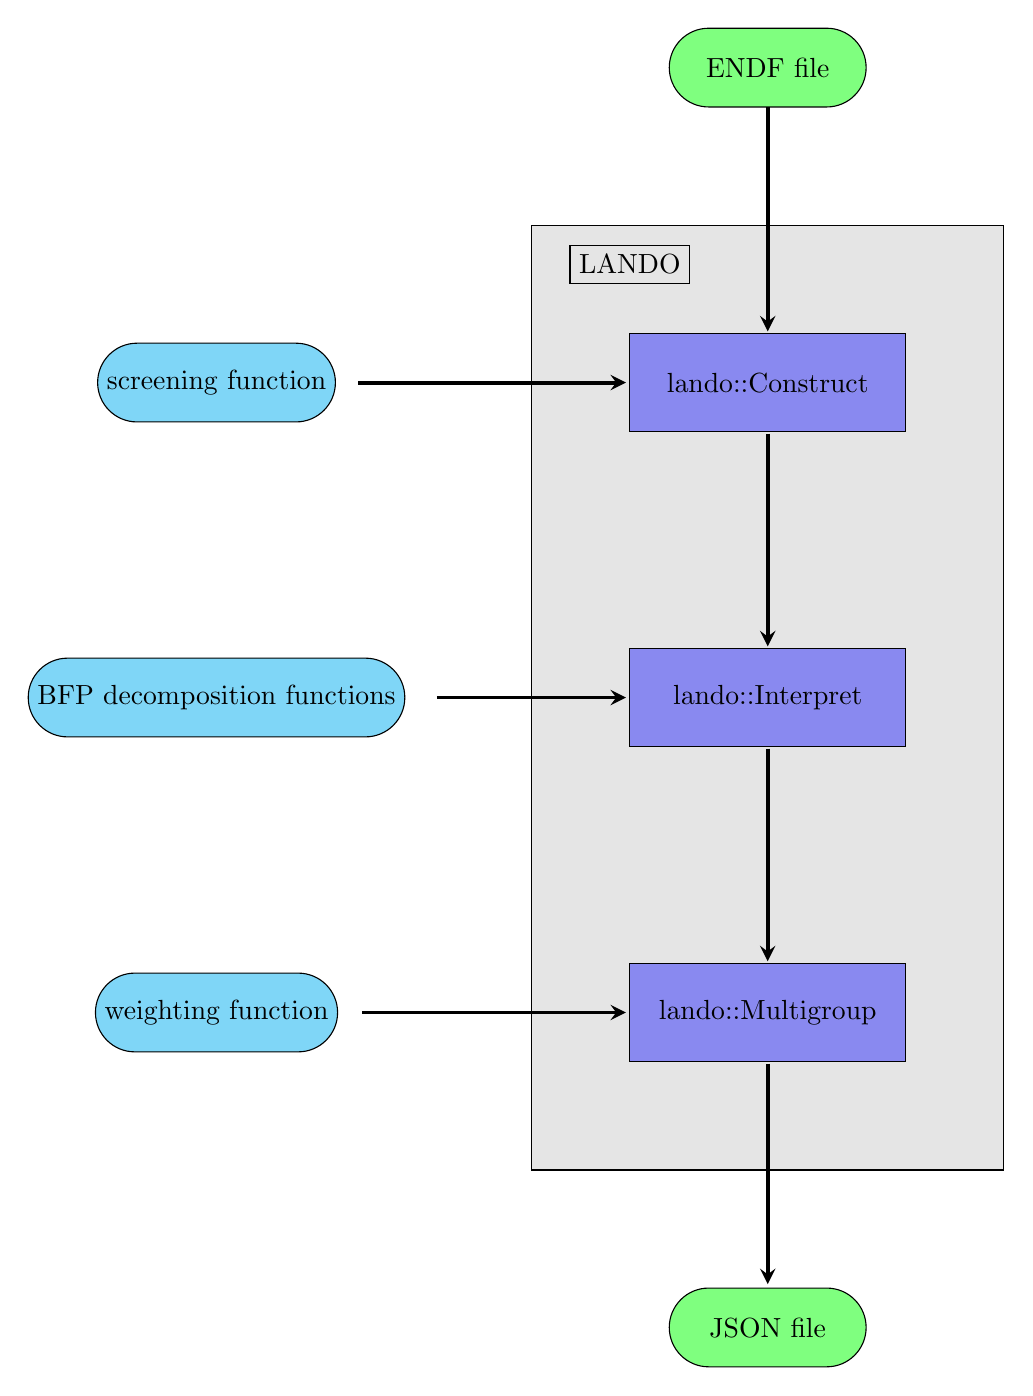
\begin{tikzpicture}
    % LANDO Code
    \node[draw,
      minimum width=6cm,
      minimum height=12cm,
      fill=lightgray,
      fill opacity=0.4] (PProcess) at (0,-4) {};
      
    % ENDF file
    \node[draw,
      rounded corners=0.5cm,
      minimum width=2.5cm,
      minimum height=1cm,
      fill=green,
      fill opacity=0.5,
      text opacity = 1] at (0,4){ENDF file};
      
    % Screening function
    \node[draw,
      rounded corners=0.5cm,
      minimum width=2.5cm,
      minimum height=1cm,
      fill=cyan,
      fill opacity=0.5,
      text opacity = 1] at (-7,0){screening function};
      
    % Construct.hpp
    \node[draw,
      minimum width=3.5cm,
      minimum height=1.25cm,
      outer sep=0,
      fill=blue,
      fill opacity=0.4,
      text opacity=1] (PProcess) at (0,0)  {lando::Construct};
    
    % BFP decomposition functions
    \node[draw,
      rounded corners=0.5cm,
      minimum width=2.5cm,
      minimum height=1cm,
      fill=cyan,
      fill opacity=0.5,
      text opacity = 1] at (-7,-4){BFP decomposition functions};
      
    % Interpret.hpp
    \node[draw,
      minimum width=3.5cm,
      minimum height=1.25cm,
      outer sep=0,
      fill=blue,
      fill opacity=0.4,
      text opacity=1] (PProcess) at (0,-4)  {lando::Interpret};
    
    % Weighting functions
    \node[draw,
      rounded corners=0.5cm,
      minimum width=2.5cm,
      minimum height=1cm,
      fill=cyan,
      fill opacity=0.5,
      text opacity = 1] at (-7,-8){weighting function};
      
    % Multigroup.hpp
    \node[draw,
      minimum width=3.5cm,
      minimum height=1.25cm,
      outer sep=0,
      fill=blue,
      fill opacity=0.4,
      text opacity=1] (PProcess) at (0,-8)  {lando::Multigroup};
    
    % JSON file
    \node[draw,
      rounded corners=0.5cm,
      minimum width=2.5cm,
      minimum height=1cm,
      fill=green,
      fill opacity=0.5,
      text opacity = 1] at (0,-12){JSON file};
    
    % Draw Arrows
    \draw[-stealth, line width=0.50mm] (0.0, 3.5) -- (0.0, 0.65);
    \draw[-stealth, line width=0.50mm] (-5.2, 0.0) -- (-1.8, 0.0);
    \draw[-stealth, line width=0.50mm] (0.0,-0.65) -- (0.0,-3.35);
    \draw[-stealth, line width=0.50mm] (-4.2,-4) -- (-1.8,-4);
    \draw[-stealth, line width=0.50mm] (0.0,-4.65) -- (0.0,-7.35);
    \draw[-stealth, line width=0.50mm] (-5.15, -8) -- (-1.8, -8);
    \draw[-stealth, line width=0.50mm] (0.0,-8.65) -- (0.0,-11.45);
    
    % Text labels
    \node[draw] at (-1.75,1.5) {LANDO};
   
  \end{tikzpicture}
\end{document}